
\chapter{Test auf realem Roboter}
\authorsection{\editortobias}

% \begin{itemize}
% 	\item Test auf realem Roboter erst spät möglich
% 	\item Schwer einzelne Komponenten zu testen da es viele Abhängigkeiten gibt
% 	\item Insbesondere der Steuerungs/Bahnplanungs/Hindernis Teil ist sowohl von den Laserscannern als auch vom Kinect-Teil abhängig.
% \end{itemize}


Nachdem die Ergebnisse der verschiedenen Gruppen in den Haupt-Entwicklungsstrang integriert sind, kann nach mehrmonatigem Testen in der Simulation mit Tests auf der realen Roboterplattform begonnen werden.

Ein Test mit \gls{hollie} zu einem früheren Zeitpunkt ist aufgrund der Abhängigkeiten zwischen den Komponenten nicht möglich.
Insbesondere das \lstinline{SegwayOmniBehaviours}-Modul, welches die Steuerung, Bahnplanung, sowie Kollisionsvermeidung übernimmt, ist beispielsweise sowohl von der Lokalisierung als auch von der Kinect abhängig.

Im Folgenden werden die Testumgebung sowie die während der Testphase aufgetretenen Schwierigkeiten beschrieben.


\section{Testumgebung}
\authorsection{\editortobias}

% \begin{itemize}
% 	\item Aufgebaute Umgebung
% 	\begin{itemize}
% 		\item FZI, oberes Stockwerk
% 		\item erste Tests in Bereich ohne Hindernisse
% 		\item Abgegrenzter Bereich zur Simulation einer Büroumgebung (Siehe Motivation!)
% 		\item Karte erstellen zur Lokalisierung
% 	\end{itemize}
% 	\item Geplantes Bewegungs-Szenario
% \end{itemize}

Als Testumgebung dient das Obergeschoss im Gebäude des \gls{fzi}.
Erste Test werden in einem weitläufigen Bereich ohne Hindernisse durchgeführt.\todoprivate{Foto?}

Für weitergehende Tests (Lokalisierug, Hindernis-Umfahrung etc.) wird ein abgegrenzter Bereich zur Simulation einer Büroumgebung eingerichtet.
Dazu werden zwei fest stehende Objekte auf einer rechtwinkligen Fläche platziert, die im entsprechenden Kartenmaterial ebenfalls verzeichnet sind, s. Abb \ref{fig:map_fzi}.
Als Hindernis dient eine einfach Plastik-Mülltonne.

\begin{figure}[h]
	\centering
	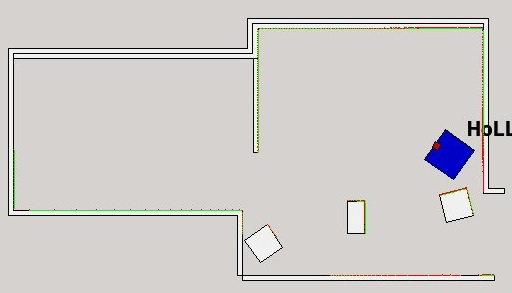
\includegraphics[width=0.6\textwidth]{graphics/map_fzi}
	\caption{Simulierte Büroumgebung für weitere Tests}
	\label{fig:map_fzi}
\end{figure}

In dieser Umgebung soll der Roboter folgendes Szenario erfüllen können:
\begin{enumerate}
  \item Person folgen ohne Hindernis
  \item Rückfahrt zum Start ohne Hindernis
  \item Pfad abfahren mit Hindernis
\end{enumerate}



\section{Aufgetretene Schwierigkeiten}
\authorsection{\editorjulian}
\todo[inline]{Julian: Schreiben}

\subsection{Laserscanner}

\begin{itemize}
	\item \glqq Unsichtbare Wand\grqq\ in ca. 4m Entfernung
	\begin{itemize}
		\item Scanner nicht exakt waagerecht angebracht
		\item nicht relevant, da Entfernung von 4m ausreichend
	\end{itemize}
	\item \glqq Tote Pixel\grqq
	\begin{itemize}
		\item Fehlmessungen werden mit Wert 0 und nicht MAX belegt
		\item Roboter steht immer im Hindernis -> keine Fortbewegung
		\item Optionale Zuschaltung der Module per XML
	\end{itemize}
\end{itemize}


\subsection{Stromversorgung}

\begin{itemize}
	\item Robotereigene Stromversorgung reicht nicht aus für Roboter + Kinect
	\item Netzgerät nötig
	\item Einschränkung der Reichweite
\end{itemize}

\subsection{Kinect}

\begin{itemize}
	\item verliert getrackten Menschen bei zu schneller Bewegung (insbesondere Rotation)
	\item Verringerung der Geschwindigkeit (Rotation sowie Translation)
\end{itemize}


\subsection{Weitere Probleme}

\begin{itemize}
	\item Odometrie auf Teppichboden
	\item SW-Bugs
	\item \ldots
\end{itemize}
